\documentclass{article}

\usepackage[dutch]{babel}
\usepackage{amsmath}
\usepackage{listings}
\usepackage{graphicx}

\setlength{\parindent}{0cm}

\title{Project Algoritmen en Datastructuren II}
\author{Jasper Van der Jeugt}
\date{\today}

\begin{document}

\maketitle
\tableofcontents

\section{Input: verschillende grafen}
Als input neemt het algoritme telkens een graaf. Daar er enorm veel
verschillende grafen bestaan, beschouwen we eerst verschillende manieren om een
graaf aan te maken, die we dan in de tests kunnen gebruiken. De verschillende
klasses die hierbij horen zitten in \verb#tests/graph#, in het java package
\verb#graph#. Ze zijn allemaal subklasses van de klasse
\verb#GraphImplementation#, die elk een specifieke constructor hebben.

\subsection{ZGraph}
Op \verb#http://zeus.ugent.be/zgraph#, een project gestart door enkele studenten
(Robrecht, Pieter en mijzelf) staan enkele voorbeeldgrafen. Om deze in te laden
is het bestandsformaat ge\"implementeerd in de klasse \verb#ZGraph#. De
constructor van deze klasse neemt een bestandsnaam, en laad deze graaf.

\subsection{CompleteGraph}
Een specifieke subklasse van de grafen zijn de complete grafen. Deze zijn zeer
makkelijk te genereren. Dit is ge\"implementeerd in de klasse
\verb#CompleteGraph#. De constructor van deze klasse neemt een getal $n$ en
maakt vervolgens de graaf $K_n$ aan.

\subsection{RandomGraph}
Voor het testen van de performantie is veel data nodig - en dus veel input. Het
zou daarom handig zijn als we willeurig grafen konden genereren met $v$ toppen
en $e$ bogen. We weten dat $e \geq v - 1$, dit is nodig als we een samenhangende
graaf willen construeren.  De klasse \verb#RandomGraph# maakt willekeurig grafen
aan met het volgende algoritme:
\newline

Neem $v$ toppen, zonder bogen. We hebben nu een onsamenhangende graaf die
bestaat uit $v$ componenten (Zie figuur \ref{fig:randomgraph-01}).
\newline

Nu gaan we in deze graaf een opspannende boom construeren. Hiervoor hebben
$v - 1$ bogen nodig. Als we deze boom eenmaal hebben, hebben we zeker een
samenhangende graaf. 
\newline

Zolang de graaf niet samenhangend is, voegen we componenten samen op de volgende
manier:
\newline

Neem twee loshangende componenten $c_1$ en $c_2$ uit de graaf. Neem in $c_1$ een
willekeurige top $v_1$ en in $c_2$ een willekeurige top $v_2$. Verbind nu $v_1$
met $v_2$. Er is nu \'e\'en component minder in de graaf. We gaan zo door tot
we een opspannende boom verkregen hebben, bijvoorbeeld deze die te zien is in
Figuur \ref{fig:randomgraph-02}.

We hebben nu $v - 1$ bogen toegevoegd. We moeten dus nog $e - v + 1$ bogen
toevoegen. Stel $E_v$ alle bogen in de complete graaf met $v$ toppen, en $T$ de
bogen in onze opspannende boom. Neem nu willekeurig $e - v + 1$ bogen uit
$E_v \setminus T$ en voeg deze toe aan onze graaf. We hebben nu een relatief
willeukeurige graaf met $e$ bogen en $v$ toppen (Voorbeeld: Figuur
\ref{fig:randomgraph-03}).

\begin{figure}
\begin{center}
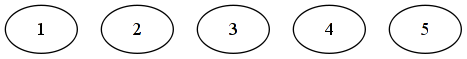
\includegraphics[width=0.6\textwidth]{images/randomgraph-01.png}
\caption{RandomGraph, stap 1}
\label{fig:randomgraph-01}
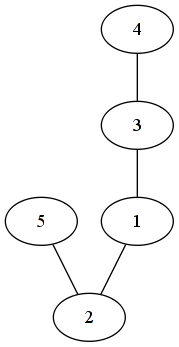
\includegraphics[width=0.3\textwidth]{images/randomgraph-02.png}
\caption{RandomGraph, stap 2}
\label{fig:randomgraph-02}
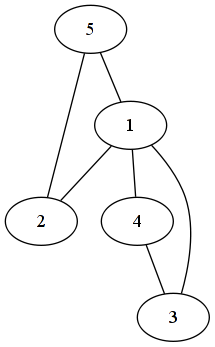
\includegraphics[width=0.3\textwidth]{images/randomgraph-03.png}
\caption{RandomGraph, stap 3}
\label{fig:randomgraph-03}
\end{center}
\end{figure}

\end{document}
